\documentclass[14pt]{extbook}
\usepackage{multicol, enumerate, enumitem, hyperref, color, soul, setspace, parskip, fancyhdr} %General Packages
\usepackage{amssymb, amsthm, amsmath, latexsym, units, mathtools} %Math Packages
\everymath{\displaystyle} %All math in Display Style
% Packages with additional options
\usepackage[headsep=0.5cm,headheight=12pt, left=1 in,right= 1 in,top= 1 in,bottom= 1 in]{geometry}
\usepackage[usenames,dvipsnames]{xcolor}
\usepackage{dashrule}  % Package to use the command below to create lines between items
\newcommand{\litem}[1]{\item#1\hspace*{-1cm}\rule{\textwidth}{0.4pt}}
\pagestyle{fancy}
\lhead{Progress Quiz 8}
\chead{}
\rhead{Version A}
\lfoot{5493-4176}
\cfoot{}
\rfoot{Summer C 2021}
\begin{document}

\begin{enumerate}
\litem{
Write the equation of the graph presented below in the form $f(x)=ax^2+bx+c$, assuming  $a=1$ or $a=-1$. Then, choose the intervals that $a, b,$ and $c$ belong to.
\begin{center}
    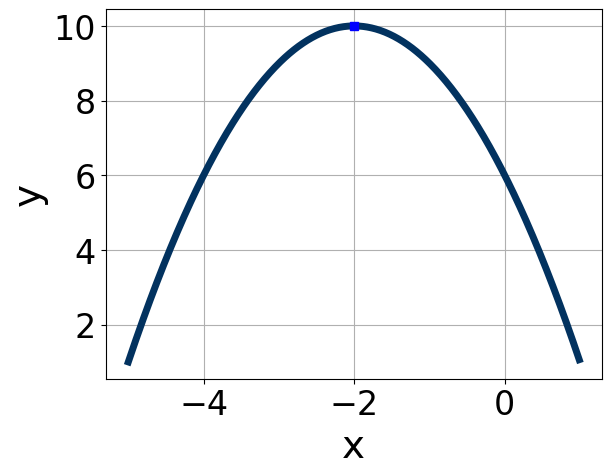
\includegraphics[width=0.5\textwidth]{../Figures/quadraticGraphToEquationA.png}
\end{center}
\begin{enumerate}[label=\Alph*.]
\item \( a \in [-2, -0.8], \hspace*{5mm} b \in [1, 6], \text{ and } \hspace*{5mm} c \in [-14, -10] \)
\item \( a \in [-2, -0.8], \hspace*{5mm} b \in [-5, -3], \text{ and } \hspace*{5mm} c \in [5, 9] \)
\item \( a \in [-2, -0.8], \hspace*{5mm} b \in [1, 6], \text{ and } \hspace*{5mm} c \in [5, 9] \)
\item \( a \in [-0.3, 1.8], \hspace*{5mm} b \in [-5, -3], \text{ and } \hspace*{5mm} c \in [11, 15] \)
\item \( a \in [-0.3, 1.8], \hspace*{5mm} b \in [1, 6], \text{ and } \hspace*{5mm} c \in [11, 15] \)

\end{enumerate} }
\litem{
Factor the quadratic below. Then, choose the intervals that contain the constants in the form $(ax+b)(cx+d); b \leq d.$\[ 54x^{2} -57 x + 10 \]\begin{enumerate}[label=\Alph*.]
\item \( a \in [1.9, 3.1], \hspace*{5mm} b \in [-6, -1], \hspace*{5mm} c \in [25.3, 27.05], \text{ and } \hspace*{5mm} d \in [-7, 4] \)
\item \( a \in [4.5, 6.5], \hspace*{5mm} b \in [-6, -1], \hspace*{5mm} c \in [7.67, 10.95], \text{ and } \hspace*{5mm} d \in [-7, 4] \)
\item \( a \in [0.8, 1.2], \hspace*{5mm} b \in [-48, -41], \hspace*{5mm} c \in [0.42, 1.12], \text{ and } \hspace*{5mm} d \in [-18, -8] \)
\item \( a \in [16.8, 19.6], \hspace*{5mm} b \in [-6, -1], \hspace*{5mm} c \in [2.05, 3.54], \text{ and } \hspace*{5mm} d \in [-7, 4] \)
\item \( \text{None of the above.} \)

\end{enumerate} }
\litem{
Solve the quadratic equation below. Then, choose the intervals that the solutions $x_1$ and $x_2$ belong to, with $x_1 \leq x_2$.\[ 10x^{2} -53 x + 36 = 0 \]\begin{enumerate}[label=\Alph*.]
\item \( x_1 \in [0.18, 0.29] \text{ and } x_2 \in [12.91, 13.59] \)
\item \( x_1 \in [0.58, 0.86] \text{ and } x_2 \in [4.23, 4.93] \)
\item \( x_1 \in [7.8, 8.15] \text{ and } x_2 \in [44.43, 45.75] \)
\item \( x_1 \in [0.85, 1.09] \text{ and } x_2 \in [3.99, 4.38] \)
\item \( x_1 \in [1.49, 1.94] \text{ and } x_2 \in [2.18, 2.4] \)

\end{enumerate} }
\litem{
Write the equation of the graph presented below in the form $f(x)=ax^2+bx+c$, assuming  $a=1$ or $a=-1$. Then, choose the intervals that $a, b,$ and $c$ belong to.
\begin{center}
    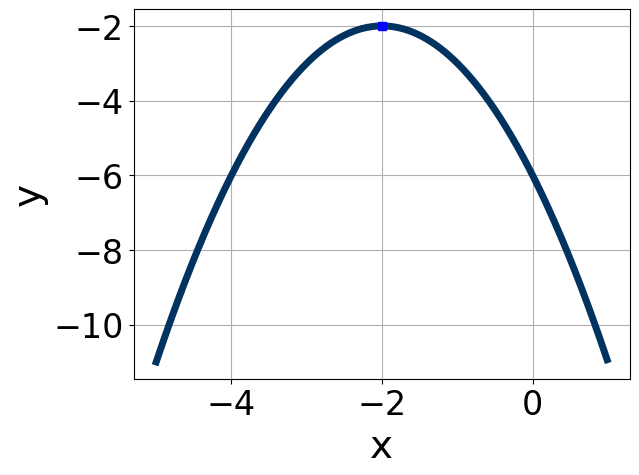
\includegraphics[width=0.5\textwidth]{../Figures/quadraticGraphToEquationCopyA.png}
\end{center}
\begin{enumerate}[label=\Alph*.]
\item \( a \in [-1.8, -0.5], \hspace*{5mm} b \in [4, 5], \text{ and } \hspace*{5mm} c \in [-4, -1] \)
\item \( a \in [0.6, 2.4], \hspace*{5mm} b \in [4, 5], \text{ and } \hspace*{5mm} c \in [-1, 3] \)
\item \( a \in [0.6, 2.4], \hspace*{5mm} b \in [-7, 1], \text{ and } \hspace*{5mm} c \in [-1, 3] \)
\item \( a \in [-1.8, -0.5], \hspace*{5mm} b \in [4, 5], \text{ and } \hspace*{5mm} c \in [-6, -4] \)
\item \( a \in [-1.8, -0.5], \hspace*{5mm} b \in [-7, 1], \text{ and } \hspace*{5mm} c \in [-6, -4] \)

\end{enumerate} }
\litem{
Solve the quadratic equation below. Then, choose the intervals that the solutions belong to, with $x_1 \leq x_2$ (if they exist).\[ 19x^{2} -13 x -8 = 0 \]\begin{enumerate}[label=\Alph*.]
\item \( x_1 \in [-1.16, -1] \text{ and } x_2 \in [0.32, 0.93] \)
\item \( x_1 \in [-0.86, 0.52] \text{ and } x_2 \in [0.53, 1.65] \)
\item \( x_1 \in [-8.02, -7.19] \text{ and } x_2 \in [20.31, 20.63] \)
\item \( x_1 \in [-27.65, -26.74] \text{ and } x_2 \in [27.96, 28.45] \)
\item \( \text{There are no Real solutions.} \)

\end{enumerate} }
\litem{
Factor the quadratic below. Then, choose the intervals that contain the constants in the form $(ax+b)(cx+d); b \leq d.$\[ 36x^{2} +60 x + 25 \]\begin{enumerate}[label=\Alph*.]
\item \( a \in [1.41, 3.78], \hspace*{5mm} b \in [5, 9], \hspace*{5mm} c \in [10.94, 13.08], \text{ and } \hspace*{5mm} d \in [4, 14] \)
\item \( a \in [17.03, 18.26], \hspace*{5mm} b \in [5, 9], \hspace*{5mm} c \in [1.93, 2.21], \text{ and } \hspace*{5mm} d \in [4, 14] \)
\item \( a \in [4.42, 6.01], \hspace*{5mm} b \in [5, 9], \hspace*{5mm} c \in [5.68, 7.39], \text{ and } \hspace*{5mm} d \in [4, 14] \)
\item \( a \in [0.67, 1.6], \hspace*{5mm} b \in [26, 37], \hspace*{5mm} c \in [0.92, 1.75], \text{ and } \hspace*{5mm} d \in [29, 31] \)
\item \( \text{None of the above.} \)

\end{enumerate} }
\litem{
Graph the equation below.\[ f(x) = -(x+1)^2 - 15 \]\begin{enumerate}[label=\Alph*.]
\begin{multicols}{2}\item 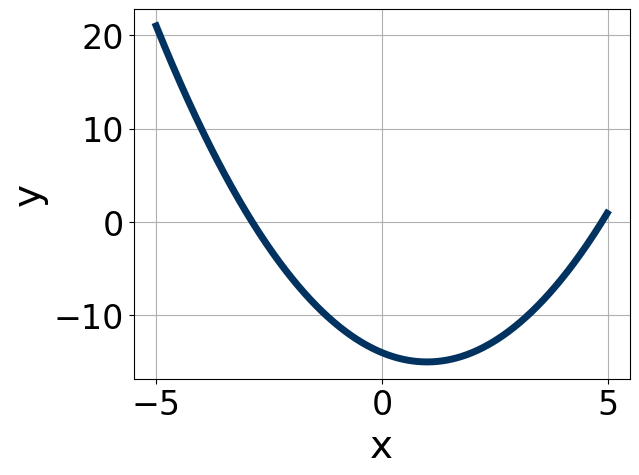
\includegraphics[width = 0.3\textwidth]{../Figures/quadraticEquationToGraphAA.png}\item 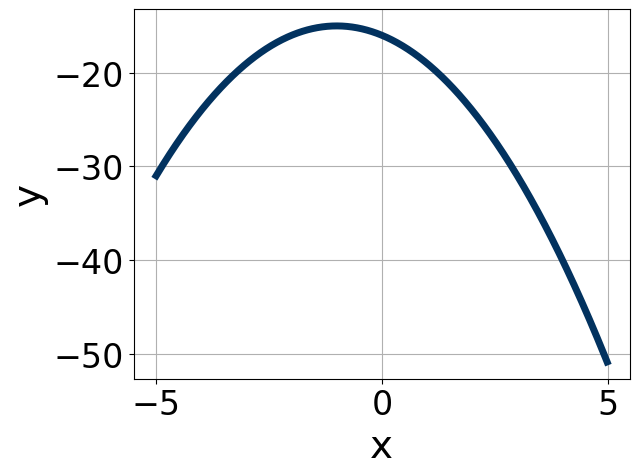
\includegraphics[width = 0.3\textwidth]{../Figures/quadraticEquationToGraphBA.png}\item 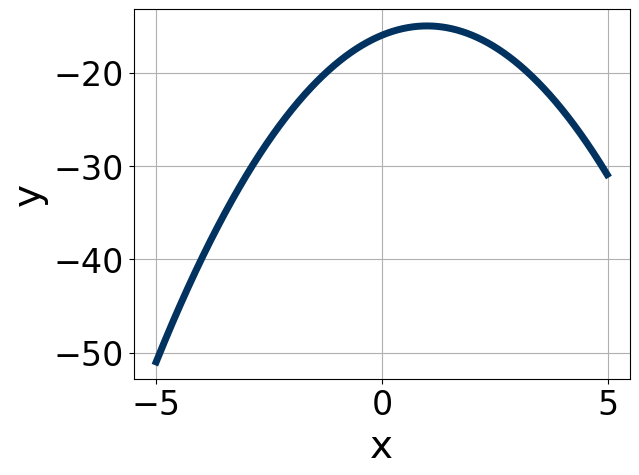
\includegraphics[width = 0.3\textwidth]{../Figures/quadraticEquationToGraphCA.png}\item 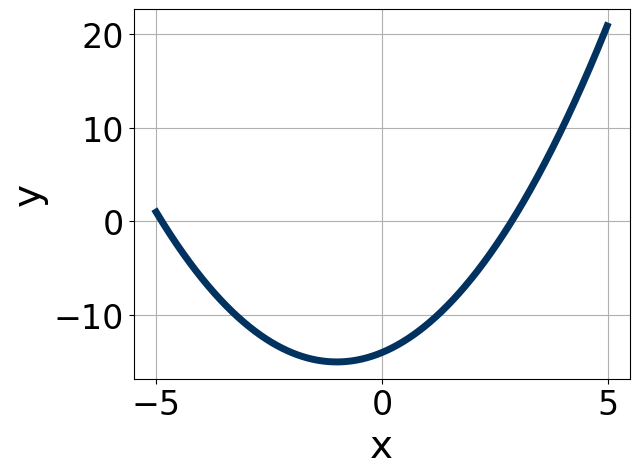
\includegraphics[width = 0.3\textwidth]{../Figures/quadraticEquationToGraphDA.png}\end{multicols}\item None of the above.
\end{enumerate} }
\litem{
Solve the quadratic equation below. Then, choose the intervals that the solutions belong to, with $x_1 \leq x_2$ (if they exist).\[ 10x^{2} +12 x -5 = 0 \]\begin{enumerate}[label=\Alph*.]
\item \( x_1 \in [-20.1, -17.9] \text{ and } x_2 \in [16.1, 18.4] \)
\item \( x_1 \in [-0.5, 1.9] \text{ and } x_2 \in [1.5, 2.7] \)
\item \( x_1 \in [-17.2, -15.1] \text{ and } x_2 \in [2.7, 5.6] \)
\item \( x_1 \in [-1.9, -0.4] \text{ and } x_2 \in [-0.6, 0.7] \)
\item \( \text{There are no Real solutions.} \)

\end{enumerate} }
\litem{
Solve the quadratic equation below. Then, choose the intervals that the solutions $x_1$ and $x_2$ belong to, with $x_1 \leq x_2$.\[ 15x^{2} +8 x -16 = 0 \]\begin{enumerate}[label=\Alph*.]
\item \( x_1 \in [-1.78, -0.94] \text{ and } x_2 \in [0.7, 1.03] \)
\item \( x_1 \in [-4.45, -3.43] \text{ and } x_2 \in [0.25, 0.36] \)
\item \( x_1 \in [-0.71, 0.61] \text{ and } x_2 \in [1.41, 1.67] \)
\item \( x_1 \in [-20.84, -18.76] \text{ and } x_2 \in [11.92, 12.11] \)
\item \( x_1 \in [-2.91, -1.6] \text{ and } x_2 \in [0.36, 0.47] \)

\end{enumerate} }
\litem{
Graph the equation below.\[ f(x) = (x+2)^2 - 15 \]\begin{enumerate}[label=\Alph*.]
\begin{multicols}{2}\item 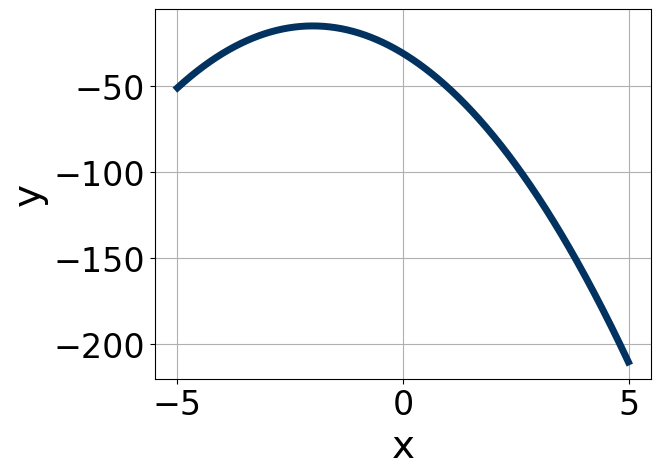
\includegraphics[width = 0.3\textwidth]{../Figures/quadraticEquationToGraphCopyAA.png}\item 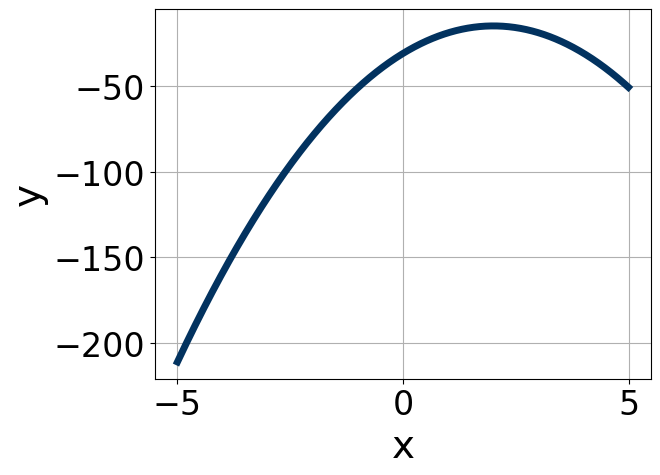
\includegraphics[width = 0.3\textwidth]{../Figures/quadraticEquationToGraphCopyBA.png}\item 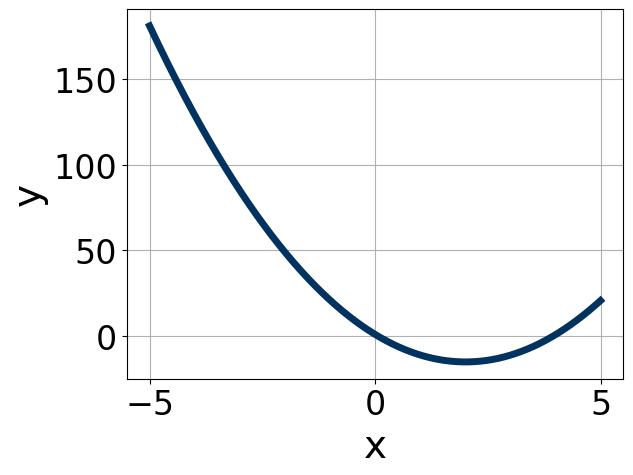
\includegraphics[width = 0.3\textwidth]{../Figures/quadraticEquationToGraphCopyCA.png}\item 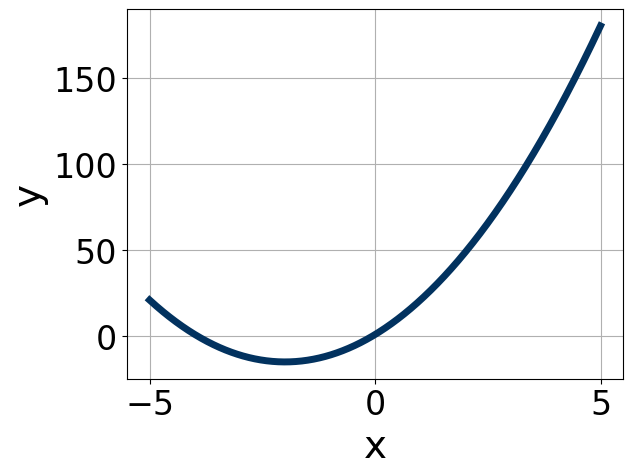
\includegraphics[width = 0.3\textwidth]{../Figures/quadraticEquationToGraphCopyDA.png}\end{multicols}\item None of the above.
\end{enumerate} }
\end{enumerate}

\end{document}